\begin{itemize}
	\item \textbf{Параметры плоской монохроматической волны:}
	\begin{itemize}
		\item $\vec{e}_p$ --- вектор поляризации
		\item $\widetilde{\vec{E}}_0 = E_0 \exp(i\varphi_0)$ --- комплексная амплитуда \\
		$\hookrightarrow$ вещественная амплитуда
		\item $\varphi(\vec{r}, t) = \omega t - \vec{k}\vec{r} + \varphi_0$ --- фаза
		\item $\varphi(t=0, \vec{r}=0) = \varphi_0$
	\end{itemize}
\end{itemize}

\begin{itemize}
	\item \textbf{Почему плоская?} 
	$\vec{k} = \begin{pmatrix} k_x \\ k_y \\ k_z \end{pmatrix} \quad \vec{r} = \begin{pmatrix} x \\ y \\ z \end{pmatrix}$
	
	$\omega t - (k_x x + k_y y + k_z z) + \varphi_0 = \text{const}$
	
	При $t = t_0$:
	$k_x x + k_y y + k_z z + C = \text{const}$ --- ур-ние плоскости, $\vec{k}$ --- нормаль к этой плоскости.
	
	$\omega t - \vec{k}\vec{r} = \text{const} \quad \Big| \dv{}{t} \implies \omega - k \dv{r_k}{t} = 0$
\end{itemize}

\begin{center}
	\begin{tikzpicture}[>=stealth]
		% Planes
		\draw[thick] (0, 0) -- ++(0, 1.5) -- ++(1, 0.5) -- ++(0, -1.5) -- cycle;
		\draw[thick] (0.5, -0.2) -- ++(0, 1.5) -- ++(1, 0.5) -- ++(0, -1.5) -- cycle;
		\draw[thick] (1, -0.4) -- ++(0, 1.5) -- ++(1, 0.5) -- ++(0, -1.5) -- cycle;
		
		\draw[->, thick] (1, 0.5) -- ++(1.5, 0) node[right] {$\vec{k}$};
		\node at (0.5, -0.8) {волновой фронт};
		
		% Vectors O, k, r
		\begin{scope}[shift={(4, 0)}]
			\draw[dashed] (-1, 0) -- (3, 0);
			\fill (0,0) circle (1.5pt) node[below] {O};
			\draw[->, thick] (0,0) -- (1.5, 0) node[below] {$\vec{k}$};
			\draw[->, thick] (0,0) -- (2, 0.8) node[above] {$\vec{r}$};
			\draw[->, thick] (2, 0.8) -- (2, 0) node[below] {$r_k$};
			\draw[->, thick] (1, 0.8) -- ++(1, 0) node[above] {$\vec{v}$};
			\draw (2, 0) rectangle (1.8, 0.2);
		\end{scope}
		
		% Wave graph
		\begin{scope}[shift={(8, -0.5)}]
			\draw[->, thick] (0,0) -- (4,0) node[right] {$r$};
			\draw[->, thick] (0,-1.5) -- (0,2) node[above] {$E$};
			\draw[thick, blue] (0, 1.5) cos (0.5, 0) sin (1, -1.5) cos (1.5, 0) sin (2, 1.5) cos (2.5, 0) sin (3, -1.5) cos (3.5, 0);
			\draw[<->] (0.05, 1.7) -- (1.95, 1.7) node[midway, above] {$\lambda$};
		\end{scope}
	\end{tikzpicture}
\end{center}

\begin{equation*}
	v_{\text{ф}} - \text{фазовая скорость} \qquad \dv{r_k}{t} = \frac{\omega}{k} \text{ --- дисперсионное соотношение}
\end{equation*}

\begin{align*}
	v_{\text{ф}} &= \frac{c}{\sqrt{\varepsilon \mu}} \text{ --- в среде} \\
	v_{\text{ф}} &= c \text{ --- в вакууме} \\
	v_{\text{ф}} &= \frac{c}{n}, \mu=1, n=\sqrt{\varepsilon} \text{ --- показатель преломления} \\
	\text{в системе СИ: } & c = \frac{1}{\sqrt{\varepsilon_0 \mu_0}} \\
	v_{\text{ф}} &= \frac{1}{\sqrt{\varepsilon \varepsilon_0 \mu \mu_0}}
\end{align*}

\subsection{Система ур-ний Максвелла для плоской монохроматической волны:}
$\rho = 0, \quad \vec{j} = 0 \qquad \qquad *(\nabla, \vec{E}) = 0, \quad \nabla = \pdv{}{x}\vec{e}_x + \pdv{}{y}\vec{e}_y + \pdv{}{z}\vec{e}_z$
\begin{equation*}
	\begin{cases}
		\operatorname{div}\vec{D} = 0 \quad (\operatorname{div}\vec{E} = 0, \text{т.к. } \vec{D} = \varepsilon\varepsilon_0\vec{E}) \\
		\operatorname{div}\vec{B} = 0 \qquad \qquad \qquad \qquad \vec{B} = \mu\mu_0\vec{H} \\
		\operatorname{rot}\vec{E} = -\pdv{\vec{B}}{t} \\
		\operatorname{rot}\vec{H} = \pdv{\vec{D}}{t}
	\end{cases}
\end{equation*}

Пусть $\vec{E} = \vec{E}_0 \exp(i(\omega t - \vec{k}\vec{r}))$ и $\vec{B} = \vec{B}_0 \exp(i(\omega t - \vec{k}\vec{r}))$.
Тогда: \\
$\pdv{\vec{E}}{t} = i\omega \underbrace{\vec{E}_0 \exp(i(\omega t - \vec{k}\vec{r}))}_{\vec{E}} = i\omega \vec{E}$ \\
$\pdv{\vec{E}}{x} = -i k_x \cdot \vec{E} \qquad \vec{k}\vec{r} = k_x x + k_y y + k_z z$

Тогда:
\begin{equation*}
	(\nabla, \vec{E}) = \pdv{E_x}{x} + \pdv{E_y}{y} + \pdv{E_z}{z} = -i k_x E_x - i k_y E_y - i k_z E_z = -i(\vec{k}, \vec{E}) = 0 \implies (\vec{k}, \vec{E}) = 0 \implies \vec{k} \perp \vec{E}
\end{equation*}
аналогично $(\vec{k}, \vec{B}) = 0 \implies \vec{k} \perp \vec{B}$.

\begin{equation*}
	\operatorname{rot}\vec{E} = \begin{vmatrix} \vec{e}_x & \vec{e}_y & \vec{e}_z \\ \pdv{}{x} & \pdv{}{y} & \pdv{}{z} \\ E_x & E_y & E_z \end{vmatrix} = \begin{vmatrix} \vec{e}_x & \vec{e}_y & \vec{e}_z \\ -ik_x & -ik_y & -ik_z \\ E_x & E_y & E_z \end{vmatrix} = -i \begin{vmatrix} \vec{e}_x & \vec{e}_y & \vec{e}_z \\ k_x & k_y & k_z \\ E_x & E_y & E_z \end{vmatrix} = -i[\vec{k}, \vec{E}]
\end{equation*}
$\hookrightarrow$ аналогично $-i[\vec{k}, \vec{H}] = -i\omega\vec{D}$

Тогда: 
\begin{align*}
	-i[\vec{k}, \vec{E}] &= -i\omega\vec{B} \quad \Big| :(-i) \\
	[\vec{k}, \vec{E}] &= \omega\vec{B}
\end{align*}
Из уравнений Максвелла: 
$\mu\mu_0[\vec{k}, \vec{H}] = -\omega\varepsilon\varepsilon_0\vec{E} \implies [\vec{k}, \vec{B}] = -\frac{\varepsilon\varepsilon_0}{\mu\mu_0}\omega\vec{E}$.

Что мы имеем уже?
\begin{equation}
	\begin{cases}
		(\vec{k}, \vec{E}) = 0 \\
		(\vec{k}, \vec{B}) = 0 \\
		[\vec{k}, \vec{E}] = \omega\vec{B} \\
		[\vec{k}, \vec{B}] = -\frac{\varepsilon\varepsilon_0}{\mu\mu_0}\omega\vec{E}
	\end{cases} \quad \leftarrow \text{ур-ния Максвелла для плоской монохроматической волны (ПМВ)}
\end{equation}

\begin{align*}
	\begin{rcases} (\vec{k}, \vec{E}) = 0 \implies \vec{k} \perp \vec{E} \\ (\vec{k}, \vec{B}) = 0 \implies \vec{k} \perp \vec{B} \end{rcases} &\implies \vec{k} \perp \vec{E} \perp \vec{B} \\
	\begin{rcases} [\vec{k}, \vec{E}] = \omega\vec{B} \implies (\vec{k}, \vec{E}, \vec{B}) \\ [\vec{k}, \vec{B}] = \varepsilon_0\varepsilon\mu\mu_0\omega\vec{E} = -\frac{\omega}{v^2}\vec{E} \end{rcases}
\end{align*}

\begin{nb}
	\textbf{Свойства ПМВ:}
	\begin{enumerate}
		\item плоская монохром. волна --- \textbf{поперечная}
		\item $\vec{k}, \vec{E}, \vec{B}$ --- \textbf{правая} тройка векторов
		\item $H = \sqrt{\frac{\varepsilon\varepsilon_0}{\mu\mu_0}} E$
	\end{enumerate}
\end{nb}

\begin{center}
	\begin{tikzpicture}[>=stealth]
		% Right hand rule system
		\draw[->] (0,0) -- (0,3) node[above] {$z$};
		\draw[->] (0,0) -- (3,0) node[right] {$y$};
		\draw[->] (0,0) -- (-2,-2) node[below left] {$x$};
		
		\draw[->, thick] (0,0) -- (0,2) node[left] {$\vec{E}$};
		\draw[->, thick] (0,0) -- (2,0) node[below] {$\vec{B}$};
		\draw[->, thick] (0,0) -- (-1.5,-1.5) node[right] {$\vec{v}_{\text{ф}}$};
		\node at (-1,-0.5) {$\vec{k}$};
		
		% Wave drawing
		\draw[thick, blue] (0,0) sin (-0.5,-0.5) cos (-1,0) sin (-1.5,0.5) cos (-2,0);
		\foreach \i in {0,-0.25,...,-2} {
			\draw[->, blue] (\i, \i) -- (\i, \i+1);
		}
		
		\begin{scope}[shift={(4, 1)}]
			\draw (0,0) rectangle (2,2);
			\draw[->, thick] (0.5,0.5) -- (1.5,0.5) node[below] {$\vec{B}$};
			\draw[->, thick] (0.5,0.5) -- (0.5,1.5) node[left] {$\vec{E}$};
			\node at (0.8, 0.8) {$\bigotimes \vec{v}_{\text{ф}}$};
		\end{scope}
	\end{tikzpicture}
\end{center}

$k = \frac{\omega}{v} \qquad k B = - \frac{\omega}{v^2} E \implies \frac{\omega}{v} B = \frac{\omega}{v^2} E \quad \text{(минус убираем, т.к. по модулю берем)} \implies E = v_{\text{ф}} B$
*в вакууме: $E = c B$.

\subsection{Интенсивность плоской монохроматической волны:}
$I = \langle |\vec{S}| \rangle_T = \frac{1}{T} \int\limits_0^T S(t) \dd{t}$, где $\vec{S} = [\vec{E}, \vec{H}]$

Пусть $\vec{k} = \begin{pmatrix} k \\ 0 \\ 0 \end{pmatrix} = k\vec{e}_x, \quad \vec{E} = \begin{pmatrix} 0 \\ E(t) \\ 0 \end{pmatrix} = E(t)\vec{e}_y, \quad \vec{H} = \begin{pmatrix} 0 \\ 0 \\ H(t) \end{pmatrix} = H(t)\vec{e}_z$

\begin{equation*}
	\vec{S} = \begin{vmatrix} \vec{e}_x & \vec{e}_y & \vec{e}_z \\ 0 & E(t) & 0 \\ 0 & 0 & H(t) \end{vmatrix} = E(t)H(t)\vec{e}_x \implies \vec{S} \upuparrows \vec{k}
\end{equation*}
$\hookrightarrow$ энергия переносится вдоль волнового вектора.

\begin{equation*}
	|\vec{S}| = E_0 \cos(\omega t - \vec{k}\vec{r}) \cdot \qty( \sqrt{\frac{\varepsilon\varepsilon_0}{\mu\mu_0}} E_0 \cos(\omega t - \vec{k}\vec{r}) ) = \sqrt{\frac{\varepsilon\varepsilon_0}{\mu\mu_0}} E_0^2 \cos^2(\omega t - \vec{k}\vec{r})
\end{equation*}

\begin{equation*}
	\langle |\vec{S}| \rangle_T = \sqrt{\frac{\varepsilon\varepsilon_0}{\mu\mu_0}} E_0^2 \underbrace{\langle \cos^2(\omega t - \vec{k}\vec{r}) \rangle_T}_{1/2}
\end{equation*}

Тогда, $I = \sqrt{\frac{\varepsilon\varepsilon_0}{\mu\mu_0}} \frac{E_0^2}{2}$

\subsection{Стоячие волны. Открытые резонаторы}

\begin{center}
	\begin{tikzpicture}[>=stealth]
		% Axis
		\draw[->] (-4,0) -- (6,0) node[right] {$z$};
		
		% Wave 1
		\draw[thick, blue] (-4,0) sin (-3,1.5) cos (-2,0) sin (-1,-1.5) cos (0,0) sin (1,1.5) cos (2,0) sin (3,-1.5) cos (4,0);
		\draw[->, thick] (-3, 2) -- (-1.5, 2) node[above, midway] {$\vec{k}_{\text{падающ.}}$};
		\draw[<-, thick] (-3, 1) -- (-1.5, 1) node[below, midway] {$\vec{k}_{\text{отраж.}}$};
		
		% Mirror
		\draw[ultra thick, fill=gray!30] (0,-2.5) rectangle (0.2,2.5);
		\node[text width=4cm, align=left] at (2, 2.5) {идеальное зеркало (проводник) --- слой металла на стекле, т.е. проводник (в металле свободные $e$)};
		\draw[->] (1.5, 2.5) -- (0.2, 1.5);
		
		\node at (0.6, -1) {$\vec{E}_0$};
		
		\begin{scope}[shift={(7,0)}]
			\draw[thick] (0,-2) -- (0,2) node[above] {$E(z<0,t)-?$};
			\node at (1, -2.2) {проводник};
			\node at (0, -2.2) {$E_0$};
			\draw[->, thick] (-1, 0.5) -- (0, 0.5) node[midway, above] {$\vec{E}_0$};
			\node at (0.2, 1) {$+$}; \node at (0.2, 0) {$+$}; \node at (0.2, -1) {$+$};
			\node at (-0.2, 1) {$-$}; \node at (-0.2, 0) {$-$}; \node at (-0.2, -1) {$-$};
			\node[text width=3cm] at (2.5, 0.5) {поле попадает в металл, $e$ колеблются с частотой как $\vec{E}$ $\hookrightarrow$ обр. волна};
			\draw[->, thick] (1, -1) -- (0, -1) node[midway, below] {$E'$};
		\end{scope}
	\end{tikzpicture}
\end{center}

$\vec{E}_{\text{падающ.}}(z<0, t) = -\vec{e}_x E_0 \exp(i(\omega t + k z)) \qquad \vec{E}_{\text{падающ.}} \upuparrows \vec{e}_x E_0 \exp(i(\omega t - k z)) \quad \vec{k} \upuparrows \vec{O}_z$ \\
$\vec{E}_z(z<0, t) = \vec{E}_{\text{пад}} + \vec{E}_{\text{отр}} = 0$ \\
$\vec{E}(z>0, t) = \vec{E}_{\text{пад}} + \vec{E}_{\text{отр}}$ \\
$\vec{E}_{\text{отр}} = -E_0 \vec{e}_x \exp(i(\omega t + k z))$

\begin{align*}
	\vec{E}(z>0, t) &= \vec{e}_x E_0 \exp(i(\omega t + k z)) - \vec{e}_x E_0 \exp(i(\omega t - k z)) \\
	&= \vec{e}_x E_0 \exp(i\omega t) \cdot \underbrace{(e^{ikz} - e^{-ikz})}_{2i \sin kz} = 2i \vec{e}_x E_0 e^{i\omega t} \sin kz
\end{align*}

$\vec{E}(z>0, t) = \Re \widetilde{\vec{E}} = \Re \qty( 2 E_0 \vec{e}_x \sin kz \cdot i(\cos\omega t + i\sin\omega t) ) = -2E_0 \vec{e}_x \sin\omega t \sin kz \qquad \hookrightarrow \text{\color{red} не бегущая волна}$

\begin{center}
	\begin{tikzpicture}[>=stealth]
		\draw[->] (0,0) -- (8,0) node[right] {$z$};
		\draw[->] (0,-2) -- (0,2) node[above] {$x$};
		
		% Envelopes
		\draw[ultra thick] (0,0) sin (1.5,1.5) cos (3,0) sin (4.5,-1.5) cos (6,0) sin (7.5,1.5);
		\draw[ultra thick, gray] (0,0) sin (1.5,-1.5) cos (3,0) sin (4.5,1.5) cos (6,0) sin (7.5,-1.5);
		
		% Intermediate steps
		\draw[thick, blue] (0,0) sin (1.5,1) cos (3,0) sin (4.5,-1) cos (6,0) sin (7.5,1);
		\draw[dashed, orange, thick] (0,0) sin (1.5,-0.5) cos (3,0) sin (4.5,0.5) cos (6,0) sin (7.5,-0.5);
		\draw[dashed, red, thick] (0,0) -- (7.5,0);
		
		\fill[orange] (0,0) circle (3pt) node[below left, text=black] {$0$};
		\fill[orange] (3,0) circle (3pt) node[below, text=black] {$\frac{\lambda}{2}$};
		\fill[orange] (6,0) circle (3pt) node[below, text=black] {$\lambda$};
		\node at (4.5, -0.5) {$\frac{3\lambda}{2}$};
		
		\node[align=left, text=red] at (5, 2) {получаем семейство кривых \\ (разные моменты времени)};
	\end{tikzpicture}
\end{center}

$k z_m = \pi m \implies z_m = \frac{\pi m}{k} = \frac{\pi m}{\frac{2\pi}{\lambda}} = \frac{\lambda}{2} m$

\noindent
\begin{minipage}{0.3\textwidth}
	\begin{tikzpicture}[>=stealth]
		\draw[thick] (0,-1.5) -- (0,1.5);
		\draw[thick] (2,-1.5) -- (2,1.5);
		\draw[<->] (0, 1.6) -- (2, 1.6) node[midway, above] {$L$};
		\draw[thick] (0,0) sin (0.5,1) cos (1,0) sin (1.5,-1) cos (2,0);
		\draw[thick] (0,0) sin (0.5,-1) cos (1,0) sin (1.5,1) cos (2,0);
		\draw[<->] (0.5, -1.2) -- (0.5, -1.8);
		\node at (0.5, -2) {пучность};
	\end{tikzpicture}
\end{minipage}
\begin{minipage}{0.65\textwidth}
	такая система зеркал \\
	называется \underline{открытый резонатор} \\
	к примеру, микроволновка --- закрытый резонатор \\
	$L = \frac{\lambda}{2} m = \frac{2\pi}{2k} m = m \frac{\pi v}{\omega} \implies$
	\begin{nb}
		$\omega_m = \frac{\pi v}{L} m$
	\end{nb}
\end{minipage}

\begin{itemize}
	\item Источник для плоской монохроматической волны --- бесконечная плоскость (в реальной жизни такого нет).
\end{itemize}

\subsection{Сферические волны}
\begin{itemize}
	\item \textbf{Сферические координаты:}
	
	\begin{minipage}{0.4\textwidth}
		\begin{tikzpicture}[>=stealth, scale=1.5]
			\draw[->] (0,0) -- (2,0) node[right] {$y$};
			\draw[->] (0,0) -- (0,2) node[above] {$z$};
			\draw[->] (0,0) -- (-1.5,-1.5) node[below left] {$x$};
			
			\draw[->, thick] (0,0) -- (1,1.5) node[right] {$r$};
			\draw[dashed] (1,1.5) -- (1,0);
			\draw[dashed] (0,0) -- (1,-1);
			\draw[dashed] (1,-1) -- (1,1.5);
			
			\draw (0,0.5) arc (90:56:0.5);
			\node at (0.2, 0.7) {$\theta$};
			
			\draw (-0.5,-0.5) arc (225:315:0.7);
			\node at (0.2, -0.6) {$\varphi$};
		\end{tikzpicture}
	\end{minipage}
	\begin{minipage}{0.5\textwidth}
		$\begin{cases} x = r \sin\theta \cos\varphi \\ y = r \sin\theta \sin\varphi \\ z = r \cos\theta \end{cases} \quad r = \sqrt{x^2 + y^2 + z^2}$
	\end{minipage}
\end{itemize}

\begin{equation*}
	\begin{cases} 
		\vec{E}(\vec{r}, t) = E(\vec{r}) \cdot \exp(i\omega t) \\ 
		(\Delta + k^2) E(\vec{r}) = 0 \quad \text{ось } y \\ 
		E(\vec{r}) = E(|\vec{r}|) \, Y(\theta, \varphi) 
	\end{cases} \quad \Delta = \frac{1}{r^2} \cdot \pdv{}{r}\qty(r^2 \pdv{}{r}) + \frac{1}{r^2 \sin\theta} \cdot \pdv{}{\theta}\qty(\sin\theta \pdv{}{\theta}) + \frac{1}{r^2 \sin^2\theta} \cdot \pdv{^2}{\varphi^2}
\end{equation*}

сферически симметричный: $Y(\theta, \varphi) = 1, \quad \pdv{}{\theta} = 0, \quad \pdv{}{\varphi} = 0$

\begin{itemize}
	\item \textbf{Ур-ние Гельмгольца:} $\frac{1}{r^2} \cdot \pdv{}{r}\qty(r^2 \cdot \pdv{E(r)}{r}) + k^2 E(r) = 0$ на больших расстояниях сферическая волна $\sim$ плоская
\end{itemize}

I решение: $E = \frac{A}{r}$ \\
подставим это:
\begin{align*}
	\frac{1}{r^2} \cdot \pdv{}{r}\qty(r^2 \cdot \pdv{}{r}\qty(\frac{A}{r})) + k^2 \cdot \frac{A}{r} &= 0 \\
	\frac{1}{r^2} \cdot \pdv{}{r}\qty(r \pdv{A}{r} - A) + k^2 \cdot \frac{A}{r} &= 0 \\
	\frac{1}{r^2} \cdot \qty( \cancel{\pdv{A}{r}} + r \pdv{^2 A}{r^2} - \cancel{\pdv{A}{r}} ) + k^2 \cdot \frac{A}{r} &= 0 \\
	\frac{1}{r} \cdot \pdv{^2 A}{r^2} + k^2 \cdot \frac{A}{r} &= 0 \\
	\pdv{^2 A}{r^2} + k^2 A &= 0 
\end{align*}

\begin{nb}
	$A(r) = C \cdot \exp(\pm i k r)$ \\
	$+$ --- волна к источнику \\
	$-$ --- волна от источника
\end{nb}

\begin{itemize}
	\item $\vec{E}(|\vec{r}|, t) = \frac{\widetilde{E}_0}{r} \cdot \exp(i(\omega t \pm k r))$ \\
	$\vec{E}(|\vec{r}|, t) = \frac{E_0}{r} \cos(\omega t \pm k r)$
\end{itemize}

\begin{center}
	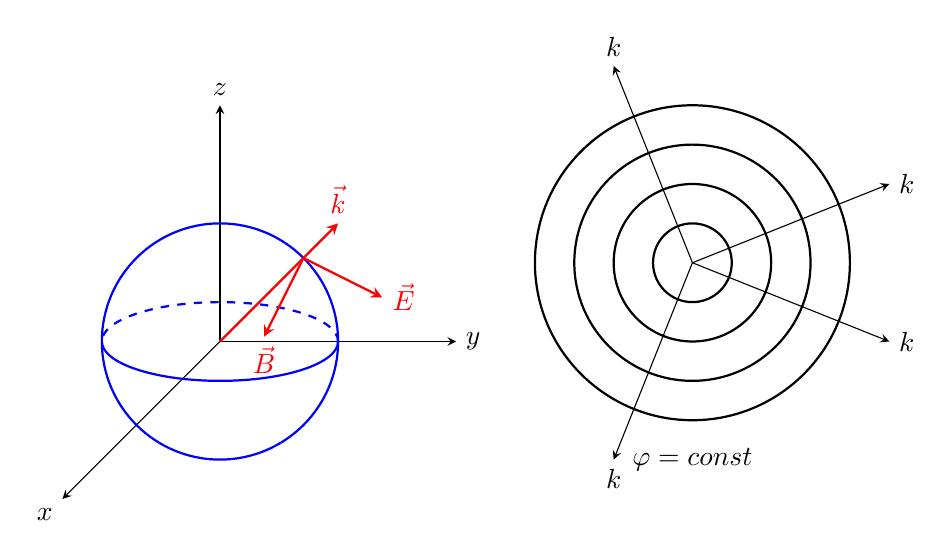
\begin{tikzpicture}[>=stealth]
		\draw[->] (0,0) -- (3,0) node[right] {$y$};
		\draw[->] (0,0) -- (0,3) node[above] {$z$};
		\draw[->] (0,0) -- (-2,-2) node[below left] {$x$};
		
		\draw[thick, blue] (0,0) circle (1.5);
		\draw[thick, blue] (-1.5,0) arc (180:360:1.5 and 0.5);
		\draw[thick, blue, dashed] (1.5,0) arc (0:180:1.5 and 0.5);
		
		\draw[->, thick, red] (0,0) -- (1.5, 1.5) node[above] {$\vec{k}$};
		\draw[->, thick, red] (1.06, 1.06) -- ++(1, -0.5) node[right] {$\vec{E}$};
		\draw[->, thick, red] (1.06, 1.06) -- ++(-0.5, -1) node[below] {$\vec{B}$};
		
		\begin{scope}[shift={(6, 1)}]
			\foreach \r in {0.5, 1, 1.5, 2} {
				\draw[thick] (0,0) circle (\r);
			}
			\draw[->] (0,0) -- (2.5, 1) node[right] {$k$};
			\draw[->] (0,0) -- (2.5, -1) node[right] {$k$};
			\draw[->] (0,0) -- (-1, 2.5) node[above] {$k$};
			\draw[->] (0,0) -- (-1, -2.5) node[below] {$k$};
			\node at (0, -2.5) {$\varphi = \text{const}$};
		\end{scope}
	\end{tikzpicture}
\end{center}

\begin{itemize}
	\item для плоской волны: $I \sim E_0^2$
	\item для сферической: $I \sim \frac{E_0^2}{r^2}$
\end{itemize}

\section{Геометрическая оптика. Распространение света в неоднородной прозрачной среде. Уравнение Эйконала. Световые лучи}

\begin{itemize}
	\item свет $\sim 10^{-7} (\lambda)$ \\
	$D \gg \lambda, \quad \lambda \to 0 \implies$ волны рассматриваем как лучи
	\item Рассмотрим свет, распространяющийся в среде, где показатель преломления неоднородный $n(r)$.
	
	$\vec{E}(\vec{r}, t) = E_0 \cdot \exp(i(\vec{k}\vec{r} - \omega t))$
	
	$k = \frac{\omega}{v} \vec{e}_s, \quad \vec{e}_s - \text{лучевой орт}, \quad n = \frac{c}{v} \implies k = \underbrace{\frac{\omega}{c}}_{k_0 - \text{волновой вектор в вакууме}} n \vec{e}_s$
	
	$\implies \vec{E}(\vec{r}, t) = E_0 \cdot \exp(i\vec{k}\vec{r} - \omega t) = E_0 \exp(i(k_0 n(r)\vec{r}\vec{e}_s - \omega t))$
	
	$\vec{E}(\vec{r}, t) = \vec{E}(\vec{r}) \cdot \exp(-i\omega t)$ \\
	$\vec{E}(\vec{r}) = a(\vec{r}) \cdot \exp(i k_0 R(\vec{r})) \quad \leftarrow \text{медленно меняющаяся функция}$ \\
	$R(\vec{r}) = n(r) \cdot \vec{r} \cdot \vec{e}_s$
	
	\item Подставим в ур-ние Гельмгольца: $(\Delta + k^2) E(\vec{r}) = 0$
\end{itemize}

\begin{equation*}
	(\Delta + k^2) a(\vec{r}) \cdot \exp(i k_0 R(\vec{r})) = 0
\end{equation*}
$\vec{\nabla} \cdot \qty[ a(\vec{r}) \cdot \exp(i k_0 R(\vec{r})) ] = (\vec{\nabla}, a) \cdot \exp(i k_0 R) + i k_0 a \vec{\nabla} R \exp(i k_0 R)$

\begin{align*}
	\Delta &= \vec{\nabla}^2 = (\vec{\nabla}^2 a) \cdot \exp(i k_0 R) + i k_0 (\vec{\nabla} a, \vec{\nabla} R) \cdot \exp(i k_0 R) \\
	&\quad + i k_0 (\vec{\nabla}^2 R) a \exp(i k_0 R) + i k_0 (\vec{\nabla} a, \vec{\nabla} R) \cdot \exp(i k_0 R) - k_0^2 a (\vec{\nabla} R)^2 \cdot \exp(i k_0 R) \equiv \\
	&\equiv (\vec{\nabla}^2 a) \exp(i k_0 R) + 2 i k_0 (\vec{\nabla} a, \vec{\nabla} R) \cdot \exp(i k_0 R) \\
	&\quad + i k_0 (\vec{\nabla}^2 R) a \cdot \exp(i k_0 R) - k_0^2 a (\vec{\nabla} R)^2 \exp(i k_0 R) \\
	&\implies \text{упрощаем } (\vec{\nabla}^2 a) \to 0
\end{align*}

$2 i k_0 (\vec{\nabla} a, \vec{\nabla} R) \cdot \exp(i k_0 R) + i k_0 (\vec{\nabla}^2 R) \cdot a \cdot \exp(i k_0 R) - k_0^2 a (\vec{\nabla} R)^2 \cdot \exp(i k_0 R)$ \\
$\Downarrow$ \\
$2 i k_0 (\vec{\nabla} a, \vec{\nabla} R) + i k_0 a (\vec{\nabla}^2 R) - k_0^2 a (\vec{\nabla} R)^2 + k_0^2 n^2 a = 0$

\begin{equation*}
	\begin{cases}
		-k_0^2 a (\vec{\nabla} R)^2 + k_0^2 n^2 a = 0 \\
		2 k_0 (\vec{\nabla} a, \vec{\nabla} R) + k_0 a (\vec{\nabla}^2 R) = 0
	\end{cases}
\end{equation*}

\begin{equation*}
	\begin{cases}
		(\vec{\nabla} R)^2 = n^2 \quad \text{\color{red} уравнение эйконала} \\
		2 (\vec{\nabla} a, \vec{\nabla} R) + a \Delta R = 0
	\end{cases}
\end{equation*}

\begin{nb}
	\textbf{Уравнение эйконала:} \qquad $\pdv{^2 R}{x^2} + \pdv{^2 R}{y^2} + \pdv{^2 R}{z^2} = n^2(x,y,z)$
\end{nb}
$\leftarrow$ описывает, как меняется волновой фронт: как в пр-ве движется фаза (поверхность постоянн. фазы); $\vec{e}_s$ --- \underline{нормаль} к этой поверхности \\
$\vec{\nabla} R = n(r)\vec{e}_s$

\noindent
\begin{minipage}{0.4\textwidth}
	любая кривая в каждой точке которой $\vec{e}_s$ направлен по касательной, явл-ся векторным полем решения ур-ния эйконала
\end{minipage}
\begin{minipage}{0.55\textwidth}
	\begin{tikzpicture}[>=stealth]
		\draw[thick] (0,-1) to[bend left=10] (0,2);
		\draw[thick] (1.5,-1) to[bend left=10] (1.5,2);
		\draw[thick] (3,-1) to[bend left=10] (3,2);
		\node at (0,-1.5) {$R_1$};
		\node at (1.5,-1.5) {$R_2$};
		\node at (3,-1.5) {$R_3$};
		
		\draw[->, thick, blue] (-1, 0) to[out=20, in=160] (4, 0) node[right, text=black] {$\vec{\nabla} R = n(\vec{r})\vec{e}_s$};
		\draw[->, thick, red] (1, 0.45) -- ++(1, 0.1) node[above] {$\vec{e}_s$};
		\node[text=black] at (2.5, 1) {касательная к лучу};
	\end{tikzpicture}
\end{minipage}

\begin{itemize}
	\item \textbf{Уравнение светового луча в неоднородной среде:}
	
	\begin{minipage}{0.2\textwidth}
		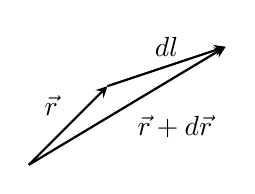
\begin{tikzpicture}[>=stealth]
			\draw[->, thick] (0,0) -- (1,1) node[midway, above left] {$\vec{r}$};
			\draw[->, thick] (1,1) -- (2.5,1.5) node[midway, above] {$dl$};
			\draw[->, thick] (0,0) -- (2.5,1.5) node[midway, below right] {$\vec{r}+d\vec{r}$};
		\end{tikzpicture}
	\end{minipage}
	\begin{minipage}{0.7\textwidth}
		из ур-ния эйконала: $\vec{n} \vec{e}_s = \vec{\nabla} R, \quad n \dv{\vec{r}}{l} = \vec{\nabla} R \quad \Big| \dv{}{l}$
		
		$d\vec{r} = \vec{e}_s dl \implies \vec{e}_s = \dv{\vec{r}}{l}$
		
		$\dv{}{l}\qty(n \dv{\vec{r}}{l}) = \dv{\vec{\nabla} R}{l} = \vec{\nabla} \qty(\dv{R}{l}) = \vec{\nabla} n$ \\
		$dR = n \vec{e}_s d\vec{r} = n \vec{e}_s \vec{e}_s dl = n dl$
	\end{minipage}
	
	\item $\dv{}{l}\qty(n \dv{\vec{r}}{l}) = \vec{\nabla} n \quad$ уравнение светового луча
	\begin{nb}
		$\dv{}{l}(n\vec{e}_s) = \vec{\nabla} n$
	\end{nb}
	
	$\dv{}{l}(n\vec{e}_s) = \vec{e}_s \dv{n}{l} + n \dv{\vec{e}_s}{l} = \vec{\nabla} n$ \\
	$\dv{\vec{e}_s}{l} = \frac{1}{n} \vec{\nabla} n - \frac{1}{n} \dv{n}{l} \vec{e}_s$ \\
	$d\vec{e}_s = \qty( \frac{1}{n} \vec{\nabla} n - \frac{1}{n} \dv{n}{l} \vec{e}_s ) dl$ --- направление орта $\vec{e}_s$
	
	луч искривляется в сторону роста $n$, в сторону более плотной среды. \\
	Если $n = \text{const}, \vec{\nabla} n = 0 \implies d\vec{e}_s = 0, \vec{e}_s = \text{const} \implies$ прямолинейное движение ({\color{red} 1 закон})
\end{itemize}

\begin{center}
	\begin{tikzpicture}[>=stealth]
		\begin{scope}[shift={(0,0)}]
			\draw[->] (0,-1.5) -- (0,1.5) node[above] {$n$};
			\draw[->] (-1.5,-1) -- (1.5,1) node[above] {$x$};
			\draw[thick, blue] (-1, 1) to[out=-60, in=180] (0.5, -0.5) to[out=0, in=200] (1.5, 0);
			\draw[->, thick, red] (-0.5, 0) -- ++(0, 0.8) node[right] {$\vec{\nabla} n$};
		\end{scope}
		
		\begin{scope}[shift={(5,0)}]
			\draw[thick] (0,0) circle (1.2);
			\node at (0,0) {земля};
			\fill (1.1, 0.5) circle (2pt) node[right] {человек};
			
			\fill[orange] (2.5, -1) circle (4pt) node[below, text=black, align=center] {солнце \\ (реальное)};
			\draw[thick, dashed] (1.1, 0.5) -- (3, 0.8) node[right, align=center] {фантомное \\ солнце \\ которое видит \\ человек};
			\draw[thick, blue] (2.5, -1) to[out=135, in=0] (1.1, 0.5);
		\end{scope}
		
		\begin{scope}[shift={(10,0)}]
			\draw[->, thick, red] (0,0) -- (3, 0.5) node[below] {$\vec{e}_s$};
			\draw[->, thick, red] (0,0) -- (1.5, 1.5);
			\draw[->, thick, red] (0,0) -- (2, -1);
			\draw[->, thick, red] (2, -1) -- (3, 0.5) node[midway, right] {$d\vec{e}_s$};
		\end{scope}
	\end{tikzpicture}
\end{center}